\documentclass[12pt]{scrartcl}
\usepackage[sexy]{james}
\usepackage[noend]{algpseudocode}
\setlength {\marginparwidth}{2cm}
\usepackage{answers}
\usepackage{array}
\usepackage{tikz}
\newenvironment{allintypewriter}{\ttfamily}{\par}
\usepackage{listings}
\usepackage{xcolor}
\usetikzlibrary{arrows.meta}
\usepackage{color}
\usepackage{mathtools}
\newcommand{\U}{\mathcal{U}}
\newcommand{\E}{\mathbb{E}}
\usetikzlibrary{arrows}
\Newassociation{hint}{hintitem}{all-hints}
\renewcommand{\solutionextension}{out}
\renewenvironment{hintitem}[1]{\item[\bfseries #1.]}{}
\renewcommand{\O}{\mathcal{O}}
\declaretheorem[style=thmbluebox,name={Chinese Remainder Theorem}]{CRT}
\renewcommand{\theCRT}{\Alph{CRT}}
\setlength\parindent{0pt}
\usepackage{sansmath}
\usepackage{pgfplots}

\usetikzlibrary{automata}
\usetikzlibrary{positioning}  %                 ...positioning nodes
\usetikzlibrary{arrows}       %                 ...customizing arrows
\newcommand{\eqdef}{=\vcentcolon}
\newcommand{\tr}{{\rm tr\ }}
\newcommand{\im}{{\rm Im\ }}
\newcommand{\spann}{{\rm span\ }}
\newcommand{\Col}{{\rm Col\ }}
\newcommand{\Row}{{\rm Row\ }}
\newcommand{\dint}{\displaystyle\int}
\newcommand{\dt}{\ {\rm d }t}
\newcommand{\PP}{\mathbb{P}}
\newcommand{\horizontal}{\par\noindent\rule{\textwidth}{0.4pt}}
\usepackage[top=3cm,left=3cm,right=3cm,bottom=3cm]{geometry}
\newcommand{\mref}[3][red]{\hypersetup{linkcolor=#1}\cref{#2}{#3}\hypersetup{linkcolor=blue}}%<<<changed

\tikzset{node distance=4.5cm, % Minimum distance between two nodes. Change if necessary.
         every state/.style={ % Sets the properties for each state
           semithick,
           fill=cyan!40},
         initial text={},     % No label on start arrow
         double distance=4pt, % Adjust appearance of accept states
         every edge/.style={  % Sets the properties for each transition
         draw,
           ->,>=stealth',     % Makes edges directed with bold arrowheads
           auto,
           semithick}}


% Start of document.
\newcommand{\sep}{\hspace*{.5em}}

\pgfplotsset{compat=1.18}
\begin{document}
\title{Computer Systems Architecture}
\author{James Zhang\thanks{Email: \mailto{jzhang72@terpmail.umd.edu}}}
\date{\today}

\definecolor{dkgreen}{rgb}{0,0.6,0}
\definecolor{gray}{rgb}{0.5,0.5,0.5}
\definecolor{mauve}{rgb}{0.58,0,0.82}

\lstset{frame=tb,
  language=Java,
  aboveskip=3mm,
  belowskip=3mm,
  showstringspaces=false,
  columns=flexible,
  basicstyle={\small\ttfamily},
  numbers=left,
  numberstyle=\tiny\color{gray},
  keywordstyle=\color{blue},
  commentstyle=\color{dkgreen},
  stringstyle=\color{mauve},
  breaklines=true,
  breakatwhitespace=true,
  tabsize=3
}


\maketitle
These are my notes for UMD's MATH411: Computer Systems Architecture. These notes are taken live in class 
(``live-\TeX``-ed). This course is taught by Professor Ilchul Yoon, whose notes are inspired by \textit{Computer Architecture:
 a Quantitative Approach} by Hennessy and Patterson.
\tableofcontents

\newpage

\section*{Computer Architecture Landscape Changes}

Here are some of the following things we will cover in the course:
\begin{itemize}
  \item How processors exploit instruction/thread/data parallelism
  \item How processors/memory work
  \item A great deal of jargon in the system area
  \item How computer architecture affects programming style
  \item How programming style affects computer architecture
\end{itemize}

\section{Chapter 1}

\begin{definition}[Dependability]
  Infrastructure providers started to offer \vocab{service level agreements} to guarantee 
  how dependable their service will be. Failure is a transition from working to not working, and 
  restoration is a transitiion from not working to working.
\end{definition}

\begin{definition}
  \vocab{Mean time to Failure (MTTF)} measures reliability, and \vocab{Failures in Time (FIT)} $ = \frac{1}{\text{MTTF}}$, 
  reported as failures per billion hours. 

  \vocab{Mean time to repair (MTTR)} measures service interruption

  \vocab{Mean time between Failures (MTBF)} = MTTF + MTTR

  \vocab{Module Availability } = MTTF / MTBF = MTTF / (MTTF + MTTR)
\end{definition}

\begin{note}
  If modules have exponentially distributed lifetimes, the age of the module does not affect 
  its probability of failure, the overall failure rate (FIT) is the sum of failure rates of the modules. 
\end{note}

\begin{example}
  See slide 8 in lecture 3 
\end{example}

\begin{definition}[Performance]
  Performance is the inverse of execution time 
  \[\text{Performance} = \frac{1}{\text{Execution Time}}\]
\end{definition}

\begin{center}
  \begin{example}
    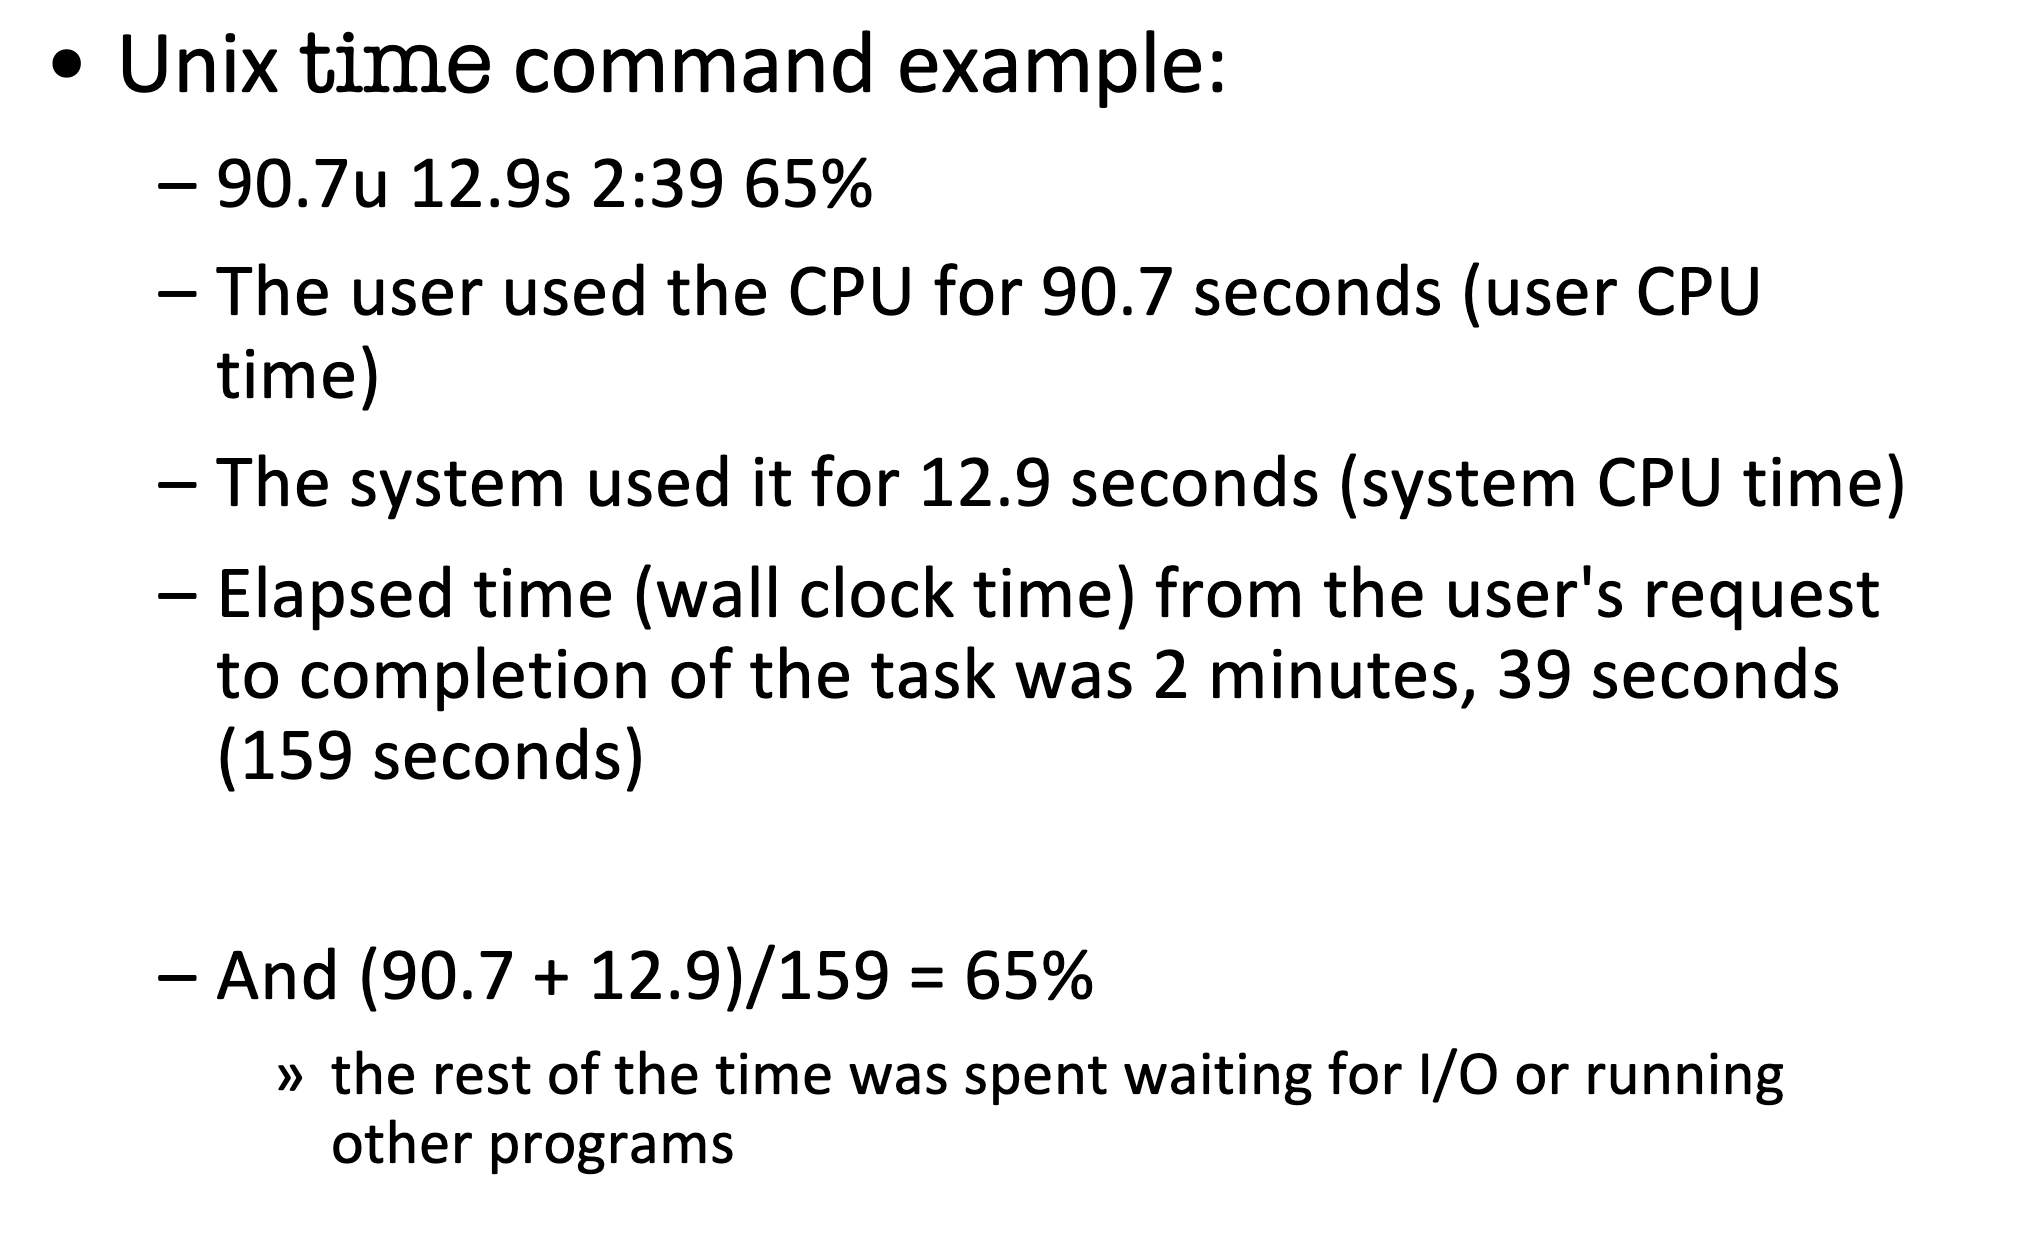
\includegraphics[width=10cm]{time.png}
  \end{example}
\end{center}

\begin{note}
  To make computers faster, make common cases faster - make addition faster, instead of optimizing the square root. 
\end{note}

\begin{definition}[Amdahl's Law]
  \vocab{Speedup} as the time the task took originally divided by the time
  the task takes after improvement

  Suppose the original task takes $1$ second, $f$ seconds in the critical piece and $1-f$ in the non-critical. 
  Then the improved task will only take $f/s$ in the critical piece, but still $1-f$ in the noncritical. Therefore, the 
  \[\text{Speedup} = \frac{\text{Old Time}}{\text{New Time}} = \frac{1}{(1-f) +\frac{f}{s}}\]
  Here $s$ is the speedup factor, note that we want to target operations that have large $f$ to maximize speedup.
\end{definition}

\begin{example}
  Suppose we get a speedup of $2$ after we replace the GPU card. If the new card can process GPU instructions $5$ times faster, 
  what is the percentage of instructions affected by the new GPU?

  \begin{proof}[Solution]
    We want to find $f$ and $s =5$ 
    \[2 = \frac{1}{(1-f) + \frac{f}{5}} \implies 2 - 2f + \frac{2f}{5} = 1 \implies \frac{-8f}{5} = -1 \implies f = \frac{5}{8} = 0.625 \]
  \end{proof}
\end{example}

\section{Appendix A}

\begin{definition}[Instruction Sets]
  Instruction sets sit in between software and hardware, and a good ISA defines how the software controls the CPU
  in a computer. Some properties of a good abstraction are 
  \begin{itemize}
    \item Lasts through many generations (portability)
    \item Generality
    \item Convenient functionality to higher levels
    \item Efficient lower level implementations
  \end{itemize}
  There are a few types of ISA classes.
  \begin{itemize}
    \item Stack - a block of memory in RAM, LIFO structure, pushing and popping
    \item Accumulator - places one operand in the accumulator (implicit) and one in memory (explicit memory address). 
    The operand in the accumulator is loaded from memory using LOAD and the result is stored in memory from the accumulator using STORE.
    \item Register (register-memory)
    \item Regsiter (load-store) - this is what MIPS uses, this ISA divides instructions into two categories: memory access and 
    (load and store between memory and registers) and ALU operations which only occur between registers. 
  \end{itemize}
\end{definition}

\begin{note}[Addressing Modes]
  See slide 57 in lecture 2.
\end{note}





\end{document}

